\section{Results}
\label{sec:results}

In this section we present parts of the outcome of our implementation.
For testing purposes, we have used 5 images together with their ground truth femur mesh.
We used the average distance and the Hausdorff distance as metrics to evaluate our fitted meshes.
The results of these evaluations can be found in \autoref{tbl:testfit}.

\begin{table}
  \centering
  \caption{Test fit distance to ground truth}
  \label{tbl:testfit}
  \begin{tabular}{lrr}
    \toprule
      \textbf{Bone Image} &
      Average Distance &
       Hausdorff Distance \\
    \midrule
      Bone 4 & 0.57 & 4.98 \\
      Bone 14 & 0.41 & 2.23 \\
      Bone 23 & 0.59 & 3.16 \\
      Bone 25 & 0.71 & 5.24 \\
      Bone 30 & 0.51 & 2.94 \\
    \midrule
      Average & 0.56 & 3.71 \\
      Standard Deviation & 0.11 & 1.33 \\
    \bottomrule
  \end{tabular}
\end{table}

We first optimized the parameters with respect to the test data.
Afterwards, we went on applying the approach to another 5 target images without ground truth.
For these, only a visual evaluation was done, as ground truth is necessary to calculate mesh distances.
One instance of the fitted result can be found in \autoref{fig:fit}.
No alarming discrepancy from the CT contours was found among all targets.

\begin{figure*}
  \centering
  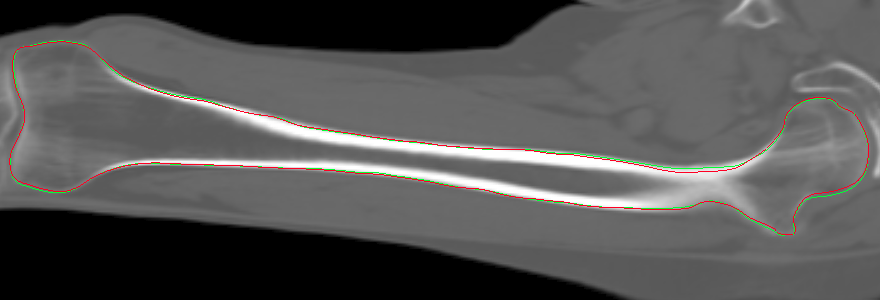
\includegraphics[width=\textwidth]{./Figures/mcmc_fit}
  \caption{
    The red contour shows the femur model fitted to the CT image in the background by our algorithm. 
    The ground truth is displayed in green to visualize the quality of the result.
  }
  \label{fig:fit}
\end{figure*}
